% Options for packages loaded elsewhere
\PassOptionsToPackage{unicode}{hyperref}
\PassOptionsToPackage{hyphens}{url}
\PassOptionsToPackage{dvipsnames,svgnames,x11names}{xcolor}
%
\documentclass[
  letterpaper,
  DIV=11,
  numbers=noendperiod]{scrartcl}

\usepackage{amsmath,amssymb}
\usepackage{iftex}
\ifPDFTeX
  \usepackage[T1]{fontenc}
  \usepackage[utf8]{inputenc}
  \usepackage{textcomp} % provide euro and other symbols
\else % if luatex or xetex
  \usepackage{unicode-math}
  \defaultfontfeatures{Scale=MatchLowercase}
  \defaultfontfeatures[\rmfamily]{Ligatures=TeX,Scale=1}
\fi
\usepackage{lmodern}
\ifPDFTeX\else  
    % xetex/luatex font selection
\fi
% Use upquote if available, for straight quotes in verbatim environments
\IfFileExists{upquote.sty}{\usepackage{upquote}}{}
\IfFileExists{microtype.sty}{% use microtype if available
  \usepackage[]{microtype}
  \UseMicrotypeSet[protrusion]{basicmath} % disable protrusion for tt fonts
}{}
\makeatletter
\@ifundefined{KOMAClassName}{% if non-KOMA class
  \IfFileExists{parskip.sty}{%
    \usepackage{parskip}
  }{% else
    \setlength{\parindent}{0pt}
    \setlength{\parskip}{6pt plus 2pt minus 1pt}}
}{% if KOMA class
  \KOMAoptions{parskip=half}}
\makeatother
\usepackage{xcolor}
\setlength{\emergencystretch}{3em} % prevent overfull lines
\setcounter{secnumdepth}{5}
% Make \paragraph and \subparagraph free-standing
\ifx\paragraph\undefined\else
  \let\oldparagraph\paragraph
  \renewcommand{\paragraph}[1]{\oldparagraph{#1}\mbox{}}
\fi
\ifx\subparagraph\undefined\else
  \let\oldsubparagraph\subparagraph
  \renewcommand{\subparagraph}[1]{\oldsubparagraph{#1}\mbox{}}
\fi


\providecommand{\tightlist}{%
  \setlength{\itemsep}{0pt}\setlength{\parskip}{0pt}}\usepackage{longtable,booktabs,array}
\usepackage{calc} % for calculating minipage widths
% Correct order of tables after \paragraph or \subparagraph
\usepackage{etoolbox}
\makeatletter
\patchcmd\longtable{\par}{\if@noskipsec\mbox{}\fi\par}{}{}
\makeatother
% Allow footnotes in longtable head/foot
\IfFileExists{footnotehyper.sty}{\usepackage{footnotehyper}}{\usepackage{footnote}}
\makesavenoteenv{longtable}
\usepackage{graphicx}
\makeatletter
\def\maxwidth{\ifdim\Gin@nat@width>\linewidth\linewidth\else\Gin@nat@width\fi}
\def\maxheight{\ifdim\Gin@nat@height>\textheight\textheight\else\Gin@nat@height\fi}
\makeatother
% Scale images if necessary, so that they will not overflow the page
% margins by default, and it is still possible to overwrite the defaults
% using explicit options in \includegraphics[width, height, ...]{}
\setkeys{Gin}{width=\maxwidth,height=\maxheight,keepaspectratio}
% Set default figure placement to htbp
\makeatletter
\def\fps@figure{htbp}
\makeatother

\KOMAoption{captions}{tableheading}
\makeatletter
\makeatother
\makeatletter
\makeatother
\makeatletter
\@ifpackageloaded{caption}{}{\usepackage{caption}}
\AtBeginDocument{%
\ifdefined\contentsname
  \renewcommand*\contentsname{Índice}
\else
  \newcommand\contentsname{Índice}
\fi
\ifdefined\listfigurename
  \renewcommand*\listfigurename{Lista de Figuras}
\else
  \newcommand\listfigurename{Lista de Figuras}
\fi
\ifdefined\listtablename
  \renewcommand*\listtablename{Lista de Tabelas}
\else
  \newcommand\listtablename{Lista de Tabelas}
\fi
\ifdefined\figurename
  \renewcommand*\figurename{Figura}
\else
  \newcommand\figurename{Figura}
\fi
\ifdefined\tablename
  \renewcommand*\tablename{Tabela}
\else
  \newcommand\tablename{Tabela}
\fi
}
\@ifpackageloaded{float}{}{\usepackage{float}}
\floatstyle{ruled}
\@ifundefined{c@chapter}{\newfloat{codelisting}{h}{lop}}{\newfloat{codelisting}{h}{lop}[chapter]}
\floatname{codelisting}{Listagem}
\newcommand*\listoflistings{\listof{codelisting}{Lista de Listagens}}
\makeatother
\makeatletter
\@ifpackageloaded{caption}{}{\usepackage{caption}}
\@ifpackageloaded{subcaption}{}{\usepackage{subcaption}}
\makeatother
\makeatletter
\@ifpackageloaded{tcolorbox}{}{\usepackage[skins,breakable]{tcolorbox}}
\makeatother
\makeatletter
\@ifundefined{shadecolor}{\definecolor{shadecolor}{rgb}{.97, .97, .97}}
\makeatother
\makeatletter
\makeatother
\makeatletter
\makeatother
\ifLuaTeX
\usepackage[bidi=basic]{babel}
\else
\usepackage[bidi=default]{babel}
\fi
\babelprovide[main,import]{portuguese}
% get rid of language-specific shorthands (see #6817):
\let\LanguageShortHands\languageshorthands
\def\languageshorthands#1{}
\ifLuaTeX
  \usepackage{selnolig}  % disable illegal ligatures
\fi
\IfFileExists{bookmark.sty}{\usepackage{bookmark}}{\usepackage{hyperref}}
\IfFileExists{xurl.sty}{\usepackage{xurl}}{} % add URL line breaks if available
\urlstyle{same} % disable monospaced font for URLs
\hypersetup{
  pdftitle={Relatório Mensal},
  pdfauthor={DIC-RF},
  pdflang={pt},
  colorlinks=true,
  linkcolor={blue},
  filecolor={Maroon},
  citecolor={Blue},
  urlcolor={Blue},
  pdfcreator={LaTeX via pandoc}}

\title{Relatório Mensal}
\usepackage{etoolbox}
\makeatletter
\providecommand{\subtitle}[1]{% add subtitle to \maketitle
  \apptocmd{\@title}{\par {\large #1 \par}}{}{}
}
\makeatother
\subtitle{Análise do IPCA - IBGE}
\author{DIC-RF}
\date{2025-08-09}

\begin{document}
\maketitle
\ifdefined\Shaded\renewenvironment{Shaded}{\begin{tcolorbox}[enhanced, boxrule=0pt, breakable, interior hidden, borderline west={3pt}{0pt}{shadecolor}, frame hidden, sharp corners]}{\end{tcolorbox}}\fi

\renewcommand*\contentsname{Índice}
{
\hypersetup{linkcolor=}
\setcounter{tocdepth}{3}
\tableofcontents
}
\hypertarget{headline}{%
\section{\texorpdfstring{\emph{Headline}}{Headline}}\label{headline}}

O IPCA do mês registrou variação de X\%, refletindo os movimentos
recentes nos preços dos principais grupos pesquisados. Destacam-se as
contribuições de alimentação, transportes e habitação, que apresentaram
comportamentos distintos em relação ao mês anterior. O resultado mantém
a inflação acumulada em 12 meses dentro do intervalo das metas
estabelecidas pelo Banco Central, indicando um cenário de estabilidade,
apesar de pressões pontuais em alguns segmentos.

\begin{figure}

{\centering 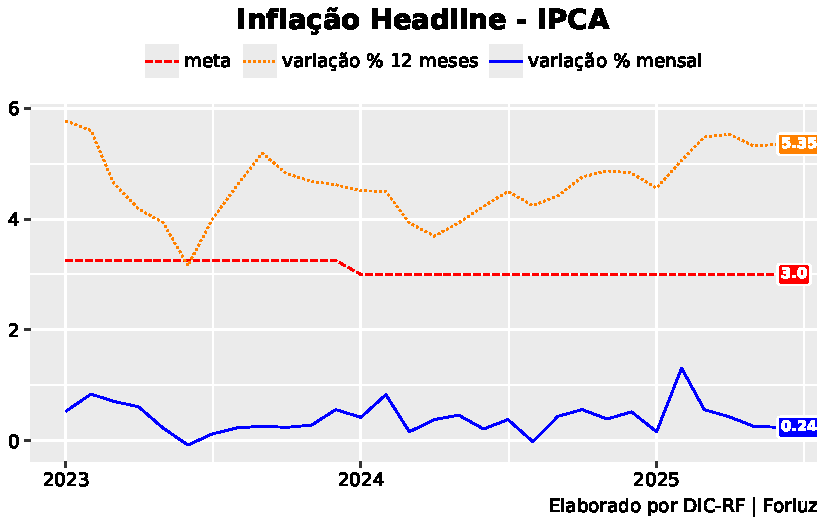
\includegraphics{IPCAForluz_files/figure-pdf/cell-5-output-1.pdf}

}

\end{figure}

\hypertarget{anuxe1lise-por-grupo-de-bens-e-serviuxe7os}{%
\section{\texorpdfstring{\emph{Análise por grupo de bens e
serviços}}{Análise por grupo de bens e serviços}}\label{anuxe1lise-por-grupo-de-bens-e-serviuxe7os}}

Em relação à variação dos itens por bens, observa-se que alguns grupos
apresentaram alta, enquanto outros registraram queda no mês analisado.
Essa dinâmica reflete fatores sazonais, choques de oferta e demanda,
além de políticas específicas que impactam determinados segmentos. A
análise detalhada por grupo permite identificar os principais vetores de
pressão ou alívio sobre o índice geral, contribuindo para uma
compreensão mais aprofundada do comportamento recente da inflação.

\begin{figure}

{\centering 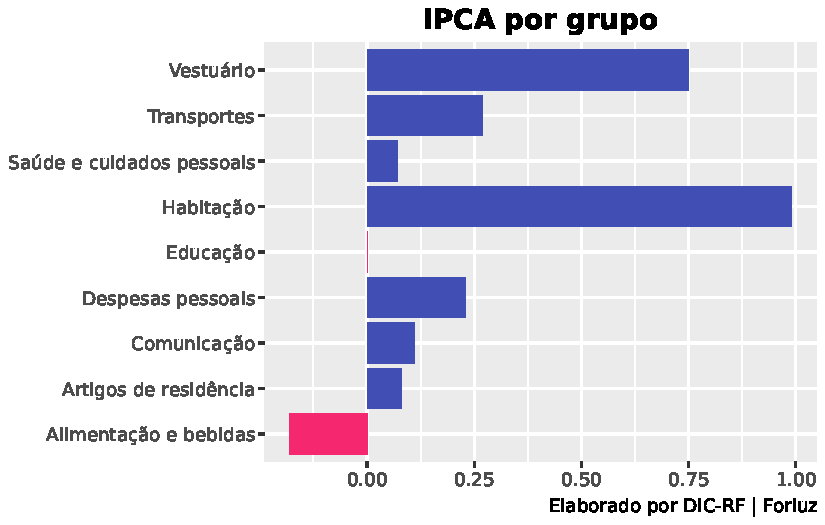
\includegraphics{IPCAForluz_files/figure-pdf/cell-6-output-1.pdf}

}

\end{figure}

\hypertarget{ponderauxe7uxe3o-por-grupo-de-itens}{%
\section{\texorpdfstring{\emph{Ponderação por grupo de
itens}}{Ponderação por grupo de itens}}\label{ponderauxe7uxe3o-por-grupo-de-itens}}

O grupo de habitação teve a principal contribuição nos preços no último
mês. Além disso, observa-se que alimentação e transportes também
apresentaram participações relevantes, refletindo movimentos específicos
desses segmentos no período analisado.

\begin{figure}

{\centering 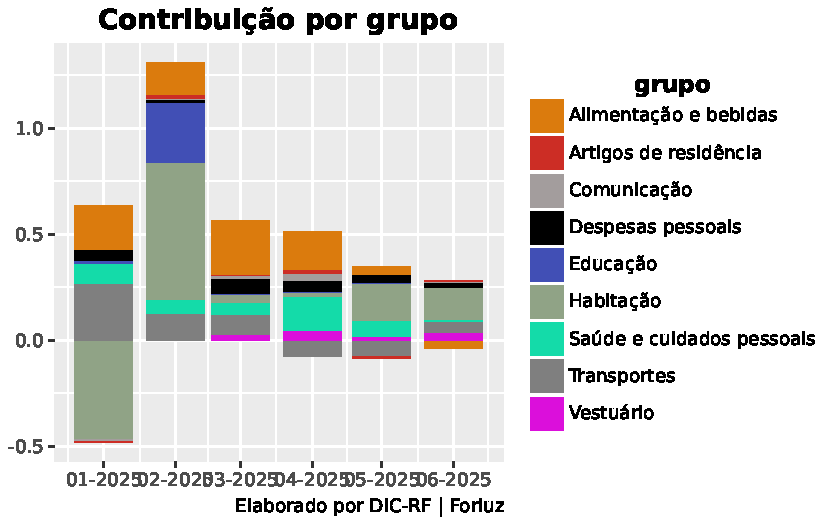
\includegraphics{IPCAForluz_files/figure-pdf/cell-7-output-1.pdf}

}

\end{figure}

\hypertarget{variauxe7uxe3o-em-12-meses-diferentes-classificauxe7uxf5es}{%
\section{\texorpdfstring{\emph{Variação em 12 meses: diferentes
classificações}}{Variação em 12 meses: diferentes classificações}}\label{variauxe7uxe3o-em-12-meses-diferentes-classificauxe7uxf5es}}

Em termos de variação por diferentes grupos de classificação observados
pelo Banco Central, vê-se uma redução da média móvel de 12 meses para
alguns itens, com destaque para o alívio em alimmentação no domicílio.
Bens industriais também respondem positivamente, em meio à apreciação do
câmbio. No entanto, os serviços continuam pressionados e sem sinais de
arrefecimento mais forte.

\begin{figure}

{\centering 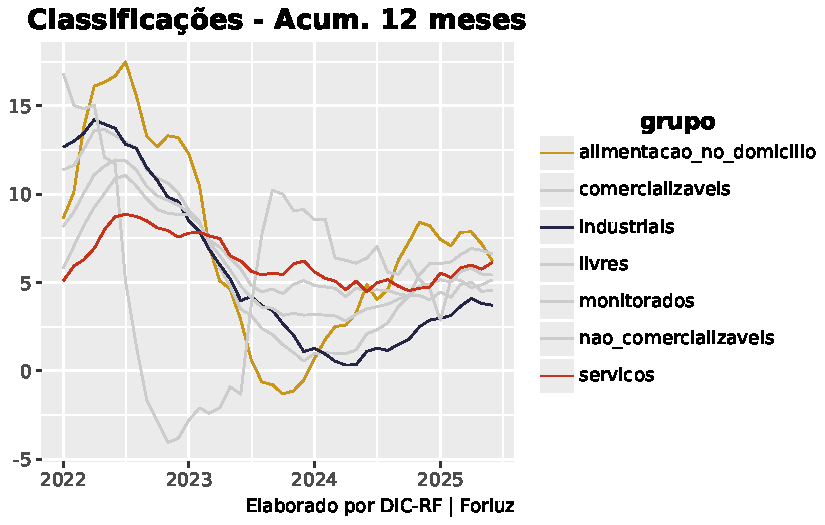
\includegraphics{IPCAForluz_files/figure-pdf/cell-8-output-1.pdf}

}

\end{figure}

\hypertarget{uxedndice-de-difusuxe3o}{%
\section{\texorpdfstring{\emph{Índice de
Difusão}}{Índice de Difusão}}\label{uxedndice-de-difusuxe3o}}

O grau de dispersão da inflação tem mostrado alívio, o que vai ao
encontro da percepção de arrefecimento inflacionário.

\begin{figure}

{\centering 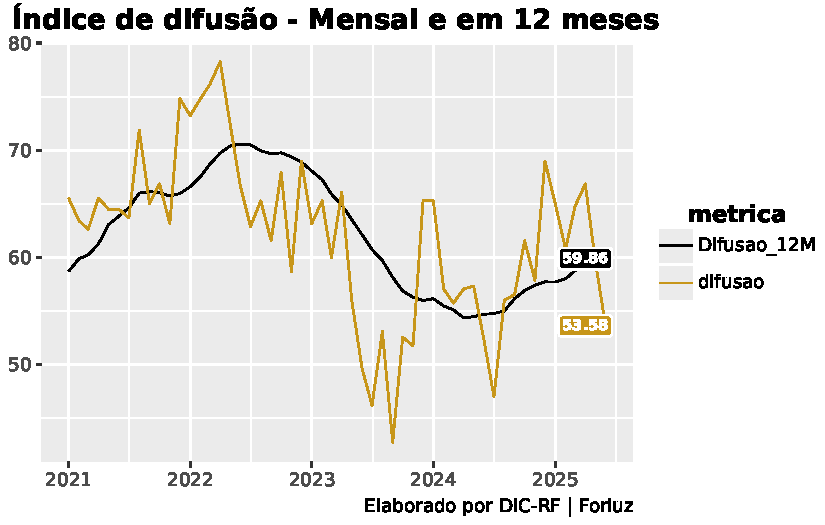
\includegraphics{IPCAForluz_files/figure-pdf/cell-9-output-1.pdf}

}

\end{figure}

\hypertarget{nuxfacleos-de-inflauxe7uxe3o---bcb}{%
\section{\texorpdfstring{\emph{Núcleos de inflação -
BCB}}{Núcleos de inflação - BCB}}\label{nuxfacleos-de-inflauxe7uxe3o---bcb}}

Os núcleos de inflação têm arrefecido. Todos eles indicaram suavização
em relação aos meses anteriores. A média dos principais núcleos segue em
trajetória de queda, refletindo o impacto do ambiente macroeconômico
mais favorável e da redução das pressões de custos. Apesar disso, alguns
componentes ainda permanecem acima do centro da meta, sugerindo cautela
na avaliação do cenário prospectivo. O comportamento benigno dos núcleos
reforça a sinalização de convergência da inflação para patamares mais
próximos do objetivo estabelecido pelo Banco Central, mas o
monitoramento contínuo segue sendo fundamental diante de possíveis
choques de oferta ou mudanças no cenário internacional.

\begin{figure}

{\centering 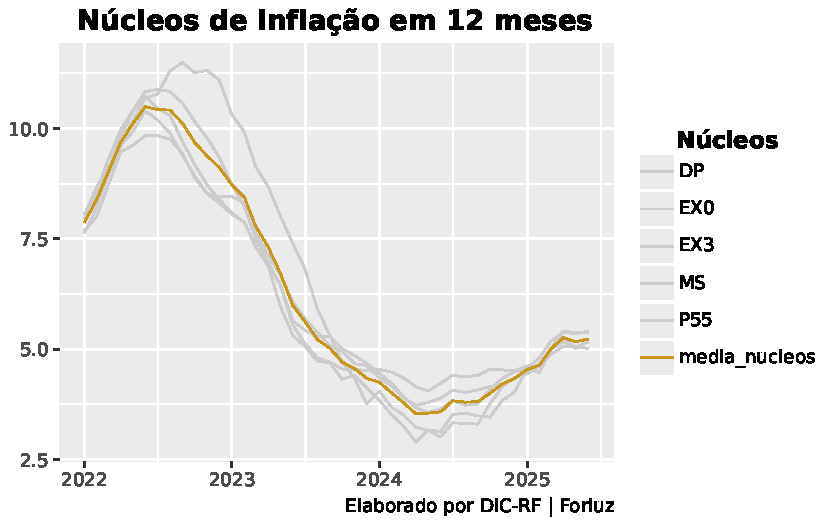
\includegraphics{IPCAForluz_files/figure-pdf/cell-10-output-1.pdf}

}

\end{figure}

\begin{figure}

{\centering 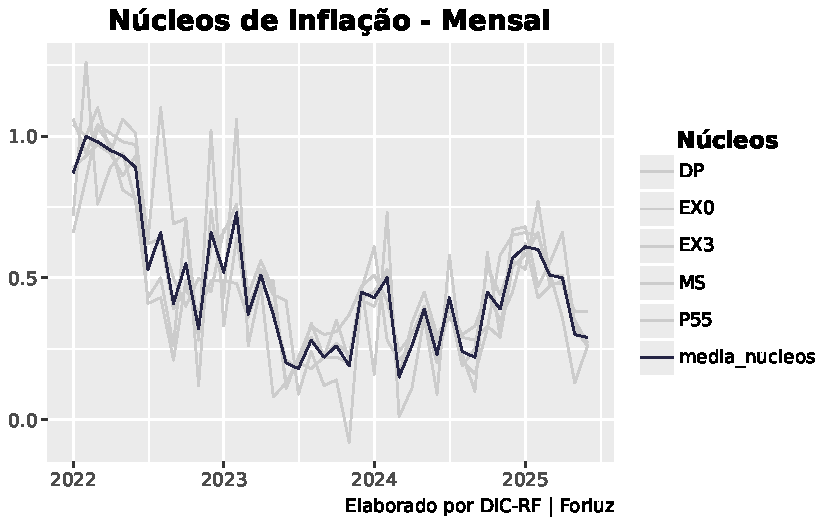
\includegraphics{IPCAForluz_files/figure-pdf/cell-11-output-1.pdf}

}

\end{figure}



\end{document}
